% The generic preamble
\documentclass[10pt,letterpaper,fleqn,titlepage]{article}

% Define packages to use
\usepackage{natbib}
\usepackage[dvips]{graphicx,color}
\usepackage{amsmath,amssymb}
\usepackage{bm}
\usepackage{caption}
\usepackage{xr}
\usepackage{ifthen}
\usepackage[dvipdfm,colorlinks,linkcolor=blue,citecolor=blue,urlcolor=blue]{hyperref}
\usepackage{fancybox}
\usepackage{textcomp}
\usepackage{alltt}
%\usepackage{floatflt}
%\usepackage{svn}


% Redefine default page
\setlength{\textheight}{9in}  % 1" above and below
\setlength{\textwidth}{6.75in}   % 0.5" left and right
\setlength{\oddsidemargin}{-0.25in}

% Redefine default paragraph
\setlength{\parindent}{0pt}
\setlength{\parskip}{1ex plus 0.5ex minus 0.2ex}

% Define caption width and default fonts
\setlength{\captionmargin}{0.5in}
\renewcommand{\captionfont}{\sffamily}
\renewcommand{\captionlabelfont}{\bfseries\sffamily}

% Define commands for super- and subscript in text mode
\newcommand{\superscript}[1]{\ensuremath{^\textrm{#1}}}
\newcommand{\subscript}[1]{\ensuremath{_\textrm{#1}}}

% Derived commands
\newcommand{\invcm}{\textrm{cm\superscript{-1}}}
\newcommand{\micron}{\ensuremath{\mu\textrm{m}}}

\newcommand{\df}{\ensuremath{\delta f}}
\newcommand{\Df}{\ensuremath{\Delta f}}
\newcommand{\dx}{\ensuremath{\delta x}}
\newcommand{\Dx}{\ensuremath{X_{max}}}
\newcommand{\Xeff}{\ensuremath{X_{eff}}}

\newcommand{\water}{\textrm{H\subscript{2}O}}
\newcommand{\carbondioxide}{\textrm{CO\subscript{2}}}
\newcommand{\ozone}{\textrm{O\subscript{3}}}

\newcommand{\taup}[1]{\ensuremath{\tau_{#1}}}
\newcommand{\efftaup}[1]{\ensuremath{\tau_{#1}^{*}}}

\newcommand{\textbfm}[1]{\boldmath\ensuremath{#1}\unboldmath}

\newcommand{\rb}[1]{\raisebox{1.5ex}[0pt]{#1}}

\newcommand{\f}[1]{\texttt{#1}}

% Define how equations are numbered
\numberwithin{equation}{section}
\numberwithin{figure}{section}
\numberwithin{table}{section}

% Define a command for title page author email footnote
\newcommand{\email}[1]
{%
  \renewcommand{\thefootnote}{\alph{footnote}}%
  \footnote{#1}
  \renewcommand{\thefootnote}{\arabic{footnote}}
}

% Define a command to print the Office Note subheading
\newcommand{\notesubheading}[1]
{%
  \ifthenelse{\equal{#1}{}}{}
  { {\Large\bfseries Office Note #1\par}%
    {\scriptsize \sc This is an unreviewed manuscript, primarily intended for informal}\\ 
    {\scriptsize \sc exchange of information among JCSDA researchers\par}%
  }
}

% Redefine the maketitle macro
\makeatletter
\def\docseries#1{\def\@docseries{#1}}
\def\docnumber#1{\def\@docnumber{#1}}
\renewcommand{\maketitle}
{%
  \thispagestyle{empty}
  \vspace*{1in}
  \begin{center}%
     \sffamily
     {\huge\bfseries Joint Center for Satellite Data Assimilation\par}%
     \notesubheading{\@docnumber}
  \end{center}
  \begin{flushleft}%
     \sffamily
     \vspace*{0.5in}
     {\Large\bfseries\ifthenelse{\equal{\@docseries}{}}{}{\@docseries: }\@title\par}%
     \medskip
     {\large\@author\par}%
     \medskip
     {\large\@date\par}%
     \bigskip\hrule\vspace*{2pc}%
  \end{flushleft}%
  \newpage
  \setcounter{footnote}{0}
}
\makeatother
\docseries{}
\docnumber{}


% Define a command for a DRAFT watermark
\usepackage{eso-pic}
\newcommand{\draftwatermark}
{
  \AddToShipoutPicture{%
    \definecolor{lightgray}{gray}{.85}
    \setlength{\unitlength}{1in}
    \put(2.5,3.5){%
      \rotatebox{45}{%
        \resizebox{4in}{1in}{%
          \textsf{\textcolor{lightgray}{DRAFT}}
        }
      }
    }
  }
}





\includeonly{srf.app,bc.app,n16.app}
% Title info
\title{AVHRR Infrared Spectral Response Function Comparison}
\author{Paul van Delst\email{paul.vandelst@noaa.gov}, David Groff\email{david.groff@noaa.gov}\\JCSDA/EMC/SAIC}
\date{October, 2008}
\docnumber{(unassigned)}
\docseries{CRTM}


%-------------------------------------------------------------------------------
%                            Ze document begins...
%-------------------------------------------------------------------------------
\begin{document}
\maketitle

%\draftwatermark

% The front matter
%=================
\thispagestyle{empty}
\vspace*{10cm}
\begin{center}
  {\sffamily\Large\bfseries Change History}
  \begin{table}[htp]
    \centering
    \begin{tabular}{|p{2cm}|p{3cm}|p{8cm}|}
      \hline
      \sffamily\textbf{Date} & \sffamily\textbf{Author} & \sffamily\textbf{Change}\\
      \hline\hline
      2008-11-01 & P.van Delst & Initial release.\\
      \hline
      2008-11-04 & P.van Delst & Minor corrections from review.\\
      \hline
      2008-11-14 & D. Groff & Added appendice for NOAA-16 cutoff issue.\\
      \hline
    \end{tabular}
  \end{table}
\end{center}
\clearpage
\pagenumbering{arabic}
\setcounter{page}{1}



\section{Introduction}
%=====================
The CRTM project is preparing to recompute all of the instrument resolution transmittances (used in the transmittance model regression fitting) to take advantage of improved spectroscopy in line-by-line (LBL) models. Additionally, we are endeavouring to use only the spectral response function (SRF) data from ``official'' sources directly related to instrument development/calibration etc.

The AVHRR SRF data used to generate the \textit{current} CRTM spectral (SpcCoeff) and transmittance model (TauCoeff) coefficients came from two sources: NOAA-15 to NOAA-17 AVHRR SRFs came from CIMSS/SSEC\footnote{Cooperative Institute for Meteorological Satellite Studies/Space Science and Engineering Center, University of Wisconsin-Madison} \citep{CIMSS_SRFs}; NOAA-18 and MetOp-A AVHRR SRFs came from \citet{Sullivan_avhrr3_n18_srf} and \citet{Sullivan_avhrr3_metop-a_srf} respectively. 
The official source of the AVHRR SRF data we wish to use for future TauCoeff generation is the  \href{http://www.star.nesdis.noaa.gov/smcd/spb/fwu/solar_cal/spec_resp_func}{NOAA AVHRR Spectral Response Function} website \citep{NESDIS_AVHRR_SRFs}.

This document describes some discrepancies we have observed during this transition period with respect to the AVHRR instrument infrared channels on the polar orbiter platforms NOAA-16, NOAA-17, NOAA-18, and MetOp-A. This lead us to question our pre-processing practices and to verify that SRF interpolation is not introducing any artifacts, such as a bias, in CRTM calculations.


\section{AVHRR infrared channel SRFs}
%====================================

\subsection{Gross SRF comparison}
%--------------------------------
Plots of the SRF data for AVHRR channels 3B, 4, and 5 for the NOAA-16 to MetOp-A platforms are shown in appendix \ref{app:srf}. SRF plots for NOAA-16 are shown in figure \ref{fig:avhrr3_n16}, NOAA-17 in figure \ref{fig:avhrr3_n17}, NOAA-18 in figure \ref{fig:avhrr3_n18}, and MetOp-A in figure \ref{fig:avhrr3_metop-a}.

In general, the SRFs shown in appendix \ref{app:srf} agree quite well. The one stand-out exception is for NOAA-17. The NESDIS/STAR and CIMSS/SSEC SRFs are completely different. It remains to be determined which set of NOAA-17 AVHRR/3 SRFs is correct.


\subsection{Interpolation differences}
%-------------------------------------
The main source of differences between the SRFs is due to interpolation. For the AVHRR instruments, the channels responses are typically reported as a function of wavelength (\micron). For the CRTM transmittance production process, we require the SRFs to be,
\begin{itemize}
  \item A function of frequency (\invcm).
  \item At a fixed frequency interval. For broadband infrared instruments, the frequency interval used is 0.1\invcm.
  \item Begun on a 0.1\invcm{} boundary such as 840.0, 900.6, etc.
\end{itemize}
As such, interpolation of the original data is required.

Our regular processing takes the original channel responses and interpolates the data using the IDL\footnote{Interactive Data Language; a scripting language that provides various functionalities for data processing and visualisation} \texttt{SPLINE} function with a tension value of 5.0, selected qualitatively. From the online IDL help\footnote{\href{http://www.ittvis.com/portals/0/pdfs/idl/refguide.pdf}{IDL Reference Guide}; for IDL Version 7.0, November 2007 Edition, see pp2346-2347; Note the download file is quite large.}:

\begin{quote}
If [the tension value] is close to 0, (e.g., .01), then effectively there is a cubic spline fit. If [the tension value] is large, (e.g., greater than 10), then the fit will be like a polynomial interpolation.
\end{quote}

The impacts of the interpolation scheme are shown visually in figures \ref{fig:avhrr3_n16.ch3.srf.zoom} and \ref{fig:avhrr3_n16.ch5.srf.zoom} for NOAA-16 AVHRR/3 channels 3 and 5; figures \ref{fig:avhrr3_n18.ch3.srf.zoom} and \ref{fig:avhrr3_n18.ch4.srf.zoom} for NOAA-18 AVHRR/3 channels 3 and 4; and in figures \ref{fig:avhrr3_metop-a.ch3.srf.zoom} and \ref{fig:avhrr3_metop-a.ch5.srf.zoom} for MetOp-A AVHRR/3 channels 3 and 5. Only two channels from each instrument are shown with the understanding that the third channel exhinbits the same sort of differences.

For NOAA-16 AVHRR/3, the current SRF data was linearly interpolated from a much lower resolution dataset, and subsequent spline interpolations have little effect. The impact of the spline interpolation on the lower resolution official SRF data is clearly evident. Note also that there is a slight vertical extent difference between the current and official SRF data that is not consistent with any type of normalisation. Closer examination of figure \ref{fig:avhrr3_n16.ch5.srf.zoom}(b) and (c) indicates that a spectral shift may describe the small differences.

In the NOAA-18 AVHRR/3 case, the SRF datasets coincide almost exactly. The differences that do remain can be attributed to the number of decimal places to which the original and intermediate data was reported in ASCII datafiles.

The current SRF data used for MetOp-A AVHRR/3 clearly suffers from quantisation of the data in the original ASCII datafile (reported to only three decimal places). This data was supplied directly by ITT \citep{Sullivan_avhrr3_metop-a_srf} and, at the time, was the only data available. The offical SRF data from \citet{NESDIS_AVHRR_SRFs} is listed as being modified on 04/21/2008, but it is not yet known if those modifications addressed the quantisation problem.

\begin{figure}[htp]
  \centering
  \includegraphics[scale=1]{graphics/zoom/avhrr3_n16.ch3.srf.zoom.eps}
  \caption{Zoom of NOAA-16 AVHRR/3 channel 3B SRF comparison. \textbf{(a)} Complete SRFs showing zoom region 1. \textbf{(b)} Magnification of SRF section from (a) showing zoom region 2.  \textbf{(c)} Magnification of SRF section from (b).}
  \label{fig:avhrr3_n16.ch3.srf.zoom}
\end{figure}

\begin{figure}[htp]
  \centering
  \includegraphics[scale=1]{graphics/zoom/avhrr3_n16.ch5.srf.zoom.eps}
  \caption{Zoom of NOAA-16 AVHRR/3 channel 5 SRF comparison. \textbf{(a)} Complete SRFs showing zoom region 1. \textbf{(b)} Magnification of SRF section from (a) showing zoom region 2.  \textbf{(c)} Magnification of SRF section from (b).}
  \label{fig:avhrr3_n16.ch5.srf.zoom}
\end{figure}

\begin{figure}[htp]
  \centering
  \includegraphics[scale=1]{graphics/zoom/avhrr3_n18.ch3.srf.zoom.eps}
  \caption{Zoom of NOAA-18 AVHRR/3 channel 3B SRF comparison. \textbf{(a)} Complete SRFs showing zoom region 1. \textbf{(b)} Magnification of SRF section from (a) showing zoom region 2.  \textbf{(c)} Magnification of SRF section from (b).}
  \label{fig:avhrr3_n18.ch3.srf.zoom}
\end{figure}

\begin{figure}[htp]
  \centering
  \includegraphics[scale=1]{graphics/zoom/avhrr3_n18.ch4.srf.zoom.eps}
  \caption{Zoom of NOAA-18 AVHRR/3 channel 4 SRF comparison. \textbf{(a)} Complete SRFs showing zoom region 1. \textbf{(b)} Magnification of SRF section from (a) showing zoom region 2.  \textbf{(c)} Magnification of SRF section from (b).}
  \label{fig:avhrr3_n18.ch4.srf.zoom}
\end{figure}


\begin{figure}[htp]
  \centering
  \includegraphics[scale=1]{graphics/zoom/avhrr3_metop-a.ch3.srf.zoom.eps}
  \caption{Zoom of MetOp-A AVHRR/3 channel 3B SRF comparison. \textbf{(a)} Complete SRFs showing zoom region 1. \textbf{(b)} Magnification of SRF section from (a) showing zoom region 2.  \textbf{(c)} Magnification of SRF section from (b).}
  \label{fig:avhrr3_metop-a.ch3.srf.zoom}
\end{figure}

\begin{figure}[htp]
  \centering
  \includegraphics[scale=1]{graphics/zoom/avhrr3_metop-a.ch5.srf.zoom.eps}
  \caption{Zoom of MetOp-A AVHRR/3 channel 5 SRF comparison. \textbf{(a)} Complete SRFs showing zoom region 1. \textbf{(b)} Magnification of SRF section from (a) showing zoom region 2.  \textbf{(c)} Magnification of SRF section from (b).}
  \label{fig:avhrr3_metop-a.ch5.srf.zoom}
\end{figure}


\section{Radiometric impact of SRF interpolation}
%================================================
To determine the radiometric impact of the various forms of the SRF (due to different data sources or different interpolation methods), effective temperatures\footnote{See appendix \ref{app:band_correction_coefficients} for a definition of effective temperature.} for each sensor channel were computed for a blackbody temperature of 285K. The result for the spline interpolated SRF with a tension of 5.0 (spline5) was chosen as the reference. Comparisons were then made with results for a linearly interpolated SRF (linear), a spline interpolated SRF with tension of 0.1 (spline0.1), a spline interpolated SRF with tension of 20 (spline20), the original uninterpolated SRF itself (original), and the current SRF used in CRTM processing (current). The temperature residuals for an SRF type, ``x'', are defined as,
\begin{equation}
  \Delta T(\textrm{x}) = T_{eff}(\textrm{spline5}) - T_{eff}(\textrm{x})
\end{equation}
and are shown in table \ref{tab:teff_comparison}. It is apparent that the type of interpolation used on the SRFs has minimal radiometric impact. Also note that the NOAA-17 $\Delta T$(current) differences in table \ref{tab:teff_comparison} indicate that, despite the very significant differences in the actual SRFs themselves (see figure \ref{fig:avhrr3_n17}), the radiometric impact of the different SRFs is still relatively low.

The computed central frequencies and band correction coefficients for the NOAA-16, -17, -18, and MetOp-A AVHRR sensors are shown in appendix \ref{app:band_correction_coefficients}.

\begin{table}[htp]
  \centering
  \begin{tabular}{l c *{6}{r@{.}l}}
    \hline
    \multicolumn{2}{c}{ } & \multicolumn{2}{c}{\textbfm{T_{eff}}} & \multicolumn{2}{c}{\textbfm{\Delta T}} & \multicolumn{2}{c}{\textbfm{\Delta T}} & \multicolumn{2}{c}{\textbfm{\Delta T}} & \multicolumn{2}{c}{\textbfm{\Delta T}} & \multicolumn{2}{c}{\textbfm{\Delta T}} \\
    \textbf{Platform} & \textbf{Channel} & \multicolumn{2}{c}{spline5} & \multicolumn{2}{c}{linear} & \multicolumn{2}{c}{spline0.1} & \multicolumn{2}{c}{spline20} & \multicolumn{2}{c}{original} & \multicolumn{2}{c}{current}\\
    \multicolumn{2}{c}{ } & \multicolumn{2}{c}{(K)} & \multicolumn{2}{c}{(K)} & \multicolumn{2}{c}{(K)} & \multicolumn{2}{c}{(K)} & \multicolumn{2}{c}{(K)}  & \multicolumn{2}{c}{(K)} \\
    \hline\hline
            &  3B & \hspace{0.2em}286&12 & -4&72e-04 &  2&04e-04 & -3&05e-04 &  1&51e-04 &  2&92e-02 \\ 
    NOAA-16 &  4  &               285&01 & -3&43e-06 &  1&73e-06 & -2&28e-06 &  1&76e-06 &  1&26e-05 \\   
            &  5  &               284&98 &  1&08e-05 & -4&00e-06 &  6&84e-06 & -3&62e-06 & -8&87e-05 \vspace{0.75em}\\ 
            &  3B &               286&13 & -4&55e-04 &  1&85e-04 & -2&91e-04 & -1&86e-03 &  6&35e-02 \\   
    NOAA-17 &  4  &               285&01 & -6&02e-06 &  2&70e-06 & -3&92e-06 & -7&89e-05 &  1&35e-03 \\   
            &  5  &               284&98 &  8&72e-06 & -3&24e-06 &  5&52e-06 &  1&60e-04 & -9&14e-04 \vspace{0.75em}\\ 
            &  3B &               286&10 & -4&45e-04 &  1&79e-04 & -2&84e-04 & -3&66e-03 & -3&91e-03 \\   
    NOAA-18 &  4  &               285&01 & -5&17e-06 &  2&29e-06 & -3&36e-06 &  1&15e-05 &  4&70e-06 \\   
            &  5  &               284&98 &  1&09e-05 & -3&91e-06 &  6&89e-06 &  6&55e-06 &  8&00e-06 \vspace{0.75em}\\ 
            &  3B &               286&33 & -4&28e-04 &  1&82e-04 & -2&75e-04 & -6&51e-03 & -8&11e-03 \\   
    MetOp-A &  4  &               285&01 & -4&68e-06 &  2&15e-06 & -3&06e-06 &  2&98e-06 &  9&08e-07 \\   
            &  5  &               284&98 &  1&17e-05 & -4&24e-06 &  7&43e-06 & -7&09e-06 & -5&24e-06 \\ 
    \hline
  \end{tabular}
  \caption{Effective temperature residuals for a blackbody temperature of 285K between the reference AVHRR SRFs (derived from the NESDIS/STAR AVHRR SRFs \citep{NESDIS_AVHRR_SRFs} via spline interpolation with tension 5.0), different interpolation methods (including none at all), and the current SRF used in CRTM processing.}
  \label{tab:teff_comparison}
\end{table}


\section{Conclusions}
%====================
This quick look at the AVHRR infrared channel SRFs can be summarised as follows:
\begin{itemize}
  \item Despite their radiometric similarity, we need to reconcile the differences between the two sets of NOAA-17 SRFs to determine which is representative of the actual instrument,
  \item The radiometric differences between the SRFs used to generate the current CRTM SpcCoeff and TauCoeff data and the official interpolated SRF are minimal, and
  \item Given any sufficiently well defined SRF, the method of interpolation used to put the SRF on a regular frequency grid has minimal radiometric impact.
\end{itemize}

% The references section
%=======================
\clearpage
\bibliographystyle{plainnat}
\bibliography{bibliography}


% Begin appendices of SRF plots
%==============================
\begin{appendix}
  \section{ATMS NPP channel SRF comparisons}
%==============================================
\label{app:srf}
This appendix plots the various NPP ATMS microwave spectral response functions (SRFs) used in this study. The "boxcar" data is derived from the data shown in table \ref{tab:atms_fo_sb_and_df}, the "Table 12" data is an edited form of the data from table 12 in reference \cite{ATMS_PFM_CalLog}, and the SDL \cite{ATMS_SRF_SDL} and NGAS \cite{ATMS_SRF_NGAS} data are digitisations of various measured ATMS channel response plots shown in reference \cite{ATMS_PFM_CalLog}.

\clearpage

% Note: the "[H]" placement option is allowed due to the use of the float package
%       in the preamble. I did this to avoid the
%        ! LaTeX Error: Too many unprocessed floats.
%       error due to the large number of figures.

\begin{figure}[H]
  \centering
  \begin{tabular}{c}
    \includegraphics[scale=1]{graphics/srf/atms_npp.ch1.srf.eps} \\
    % the hand-crafted legend
    \setlength{\unitlength}{1cm}
    \begin{picture}(2.0,0.0)(0.0,-2.0)
      \thicklines
      \color{green}
      \put(0.0,0.7 ){\line(1,0){1}}
      \put(1.1,0.55){\sffamily SDL}
      \color{red}
      \put(0.0,1.2 ){\line(1,0){1}}
      \put(1.1,1.05){\sffamily Table 12}
      \color{black}
      \put(0.0,1.7 ){\line(1,0){1}}
      \put(1.1,1.55){\sffamily Boxcar}
    \end{picture} \\\\
    \includegraphics[bb=249 194 1431 1035,scale=0.3]{graphics/log_book/ch1.eps}
  \end{tabular}
  \caption{NPP ATMS channel 1 response. \textbf{(Top)} Boxcar and digitised data. \textbf{(Bottom)} Nominal filter response from ATMS Calibration Data Book\cite{ATMS_PFM_CalLog}.}
  \label{fig:atms_npp.ch1.srf}
\end{figure}

\begin{figure}[H]
  \centering
  \includegraphics[scale=1]{graphics/srf/atms_npp.ch2.srf.eps}
  % the hand-crafted legend
  \setlength{\unitlength}{1cm}
  \begin{picture}(2.0,0.0)(0.0,-2.0)
    \thicklines
    \color{red}
    \put(0.0,1.2 ){\line(1,0){1}}
    \put(1.1,1.05){\sffamily Table 12}
    \color{black}
    \put(0.0,1.7 ){\line(1,0){1}}
    \put(1.1,1.55){\sffamily Boxcar}
  \end{picture}
  \caption{NPP ATMS channel 2 response.}
  \label{fig:atms_npp.ch2.srf}
\end{figure}

\begin{figure}[H]
  \centering
  \includegraphics[scale=1]{graphics/srf/atms_npp.ch3.srf.eps}
  % the hand-crafted legend
  \setlength{\unitlength}{1cm}
  \begin{picture}(2.0,0.0)(0.0,-2.0)
    \thicklines
    \color{red}
    \put(0.0,1.2 ){\line(1,0){1}}
    \put(1.1,1.05){\sffamily Table 12}
    \color{black}
    \put(0.0,1.7 ){\line(1,0){1}}
    \put(1.1,1.55){\sffamily Boxcar}
  \end{picture}
  \caption{NPP ATMS channel 3 response.}
  \label{fig:atms_npp.ch3.srf}
\end{figure}

\begin{figure}[H]
  \centering
  \begin{tabular}{c}
    \includegraphics[scale=1]{graphics/srf/atms_npp.ch4.srf.eps} \\
    % the hand-crafted legend
    \setlength{\unitlength}{1cm}
    \begin{picture}(2.0,0.0)(0.0,-2.0)
      \thicklines
      \color{blue}
      \put(0.0,0.7 ){\line(1,0){1}}
      \put(1.1,0.55){\sffamily NGAS}
      \color{red}
      \put(0.0,1.2 ){\line(1,0){1}}
      \put(1.1,1.05){\sffamily Table 12}
      \color{black}
      \put(0.0,1.7 ){\line(1,0){1}}
      \put(1.1,1.55){\sffamily Boxcar}
    \end{picture} \\\\
    \includegraphics[bb=249 194 1431 1035,scale=0.3]{graphics/log_book/ch4.eps}
  \end{tabular}
  \caption{NPP ATMS channel 4 response. \textbf{(Top)} Boxcar and digitised data. \textbf{(Bottom)} Nominal filter response from ATMS Calibration Data Book\cite{ATMS_PFM_CalLog}.}
  \label{fig:atms_npp.ch4.srf}
\end{figure}

\begin{figure}[H]
  \centering
  \begin{tabular}{c}
    \includegraphics[scale=1]{graphics/srf/atms_npp.ch5.srf.eps} \\
    % the hand-crafted legend
    \setlength{\unitlength}{1cm}
    \begin{picture}(2.0,0.0)(0.0,-2.0)
      \thicklines
      \color{blue}
      \put(0.0,0.7 ){\line(1,0){1}}
      \put(1.1,0.55){\sffamily NGAS}
      \color{red}
      \put(0.0,1.2 ){\line(1,0){1}}
      \put(1.1,1.05){\sffamily Table 12}
      \color{black}
      \put(0.0,1.7 ){\line(1,0){1}}
      \put(1.1,1.55){\sffamily Boxcar}
    \end{picture} \\\\
    \includegraphics[bb=249 194 1431 1035,scale=0.3]{graphics/log_book/ch5.eps}
  \end{tabular}
  \caption{NPP ATMS channel 5 response. \textbf{(Top)} Boxcar and digitised data. \textbf{(Bottom)} Nominal filter response from ATMS Calibration Data Book\cite{ATMS_PFM_CalLog}.}
  \label{fig:atms_npp.ch5.srf}
\end{figure}

\begin{figure}[H]
  \centering
  \includegraphics[scale=1]{graphics/srf/atms_npp.ch6.srf.eps}
  % the hand-crafted legend
  \setlength{\unitlength}{1cm}
  \begin{picture}(2.0,0.0)(3.0,-2.0)
    \thicklines
    \color{red}
    \put(0.0,1.2 ){\line(1,0){1}}
    \put(1.1,1.05){\sffamily Table 12}
    \color{black}
    \put(0.0,1.7 ){\line(1,0){1}}
    \put(1.1,1.55){\sffamily Boxcar}
  \end{picture}
  \caption{NPP ATMS channel 6 response.}
  \label{fig:atms_npp.ch6.srf}
\end{figure}

\begin{figure}[H]
  \centering
  \includegraphics[scale=1]{graphics/srf/atms_npp.ch7.srf.eps}
  % the hand-crafted legend
  \setlength{\unitlength}{1cm}
  \begin{picture}(2.0,0.0)(0.0,-2.0)
    \thicklines
    \color{red}
    \put(0.0,1.2 ){\line(1,0){1}}
    \put(1.1,1.05){\sffamily Table 12}
    \color{black}
    \put(0.0,1.7 ){\line(1,0){1}}
    \put(1.1,1.55){\sffamily Boxcar}
  \end{picture}
  \caption{NPP ATMS channel 7 response.}
  \label{fig:atms_npp.ch7.srf}
\end{figure}

\begin{figure}[H]
  \centering
  \includegraphics[scale=1]{graphics/srf/atms_npp.ch8.srf.eps}
  % the hand-crafted legend
  \setlength{\unitlength}{1cm}
  \begin{picture}(2.0,0.0)(0.0,-2.0)
    \thicklines
    \color{red}
    \put(0.0,1.2 ){\line(1,0){1}}
    \put(1.1,1.05){\sffamily Table 12}
    \color{black}
    \put(0.0,1.7 ){\line(1,0){1}}
    \put(1.1,1.55){\sffamily Boxcar}
  \end{picture}
  \caption{NPP ATMS channel 8 response.}
  \label{fig:atms_npp.ch8.srf}
\end{figure}

\begin{figure}[H]
  \centering
  \begin{tabular}{c}
    \includegraphics[scale=1]{graphics/srf/atms_npp.ch9.srf.eps} \\
    % the hand-crafted legend
    \setlength{\unitlength}{1cm}
    \begin{picture}(2.0,0.0)(0.0,-2.0)
      \thicklines
      \color{blue}
      \put(0.0,0.7 ){\line(1,0){1}}
      \put(1.1,0.55){\sffamily NGAS}
      \color{red}
      \put(0.0,1.2 ){\line(1,0){1}}
      \put(1.1,1.05){\sffamily Table 12}
      \color{black}
      \put(0.0,1.7 ){\line(1,0){1}}
      \put(1.1,1.55){\sffamily Boxcar}
    \end{picture} \\\\
    \includegraphics[bb=249 194 1431 1035,scale=0.3]{graphics/log_book/ch9.eps}
  \end{tabular}
  \caption{NPP ATMS channel 9 response. \textbf{(Top)} Boxcar and digitised data. \textbf{(Bottom)} Nominal filter response from ATMS Calibration Data Book\cite{ATMS_PFM_CalLog}.}
  \label{fig:atms_npp.ch9.srf}
\end{figure}

\begin{figure}[H]
  \centering
  \includegraphics[scale=1]{graphics/srf/atms_npp.ch10.srf.eps}
  % the hand-crafted legend
  \setlength{\unitlength}{1cm}
  \begin{picture}(2.0,0.0)(0.0,-2.0)
    \thicklines
    \color{red}
    \put(0.0,1.2 ){\line(1,0){1}}
    \put(1.1,1.05){\sffamily Table 12}
    \color{black}
    \put(0.0,1.7 ){\line(1,0){1}}
    \put(1.1,1.55){\sffamily Boxcar}
  \end{picture}
  \caption{NPP ATMS channel 10 response.}
  \label{fig:atms_npp.ch10.srf}
\end{figure}

\begin{figure}[H]
  \centering
  \includegraphics[scale=1]{graphics/srf/atms_npp.ch11.srf.eps}
  % the hand-crafted legend
  \setlength{\unitlength}{1cm}
  \begin{picture}(2.0,0.0)(3.5,-2.0)
    \thicklines
    \color{red}
    \put(0.0,1.2 ){\line(1,0){1}}
    \put(1.1,1.05){\sffamily Table 12}
    \color{black}
    \put(0.0,1.7 ){\line(1,0){1}}
    \put(1.1,1.55){\sffamily Boxcar}
  \end{picture}
  \caption{NPP ATMS channel 11 response.}
  \label{fig:atms_npp.ch11.srf}
\end{figure}

\begin{figure}[H]
  \centering
  \begin{tabular}{c c}
    \multicolumn{2}{c}{\includegraphics[scale=1]{graphics/srf/atms_npp.ch12.srf.eps}}\\
    % the hand-crafted legend
    \multicolumn{2}{c}{
      \setlength{\unitlength}{1cm}
      \begin{picture}(2.0,0.0)(1.7,-1.2)
        \thicklines
        \color{green}
        \put(0.0,0.7 ){\line(1,0){1}}
        \put(1.1,0.55){\sffamily SDL}
        \color{red}
        \put(0.0,1.2 ){\line(1,0){1}}
        \put(1.1,1.05){\sffamily Table 12}
        \color{black}
        \put(0.0,1.7 ){\line(1,0){1}}
        \put(1.1,1.55){\sffamily Boxcar}
      \end{picture}} \\\\
    \includegraphics[bb=249 194 1431 1035,scale=0.2]{graphics/log_book/ch12_lowf.eps} & 
    \includegraphics[bb=249 194 1431 1035,scale=0.2]{graphics/log_book/ch12_hif.eps}
  \end{tabular}
  \caption{NPP ATMS channel 12 response. \textbf{(Top)} Boxcar and digitised data. \textbf{(Bottom)} Nominal filter (low and high IF) response from ATMS Calibration Data Book\cite{ATMS_PFM_CalLog}. The low IF (left) reponsse corresponds to band \#3 and the high IF (right) response to band \#4.}
  \label{fig:atms_npp.ch12.srf}
\end{figure}

\begin{figure}[H]
  \centering
  \begin{tabular}{c c}
    \multicolumn{2}{c}{\includegraphics[scale=1]{graphics/srf/atms_npp.ch13.srf.eps}}\\
    % the hand-crafted legend
    \multicolumn{2}{c}{
      \setlength{\unitlength}{1cm}
      \begin{picture}(2.0,0.0)(1.7,-1.6)
        \thicklines
        \color{blue}
        \put(0.0,0.2 ){\line(1,0){1}}
        \put(1.1,0.05){\sffamily NGAS}
        \color{green}
        \put(0.0,0.7 ){\line(1,0){1}}
        \put(1.1,0.55){\sffamily SDL}
        \color{red}
        \put(0.0,1.2 ){\line(1,0){1}}
        \put(1.1,1.05){\sffamily Table 12}
        \color{black}
        \put(0.0,1.7 ){\line(1,0){1}}
        \put(1.1,1.55){\sffamily Boxcar}
      \end{picture}} \\\\
    \includegraphics[bb=249 194 1431 1035,scale=0.2]{graphics/log_book/ch13_lowf.eps} & 
    \includegraphics[bb=249 194 1431 1035,scale=0.2]{graphics/log_book/ch13_hif.eps}
  \end{tabular}
  \caption{NPP ATMS channel 13 response. \textbf{(Top)} Boxcar and digitised data. \textbf{(Bottom)} Nominal filter (low and high IF) response from ATMS Calibration Data Book\cite{ATMS_PFM_CalLog}. The low IF (left) reponsse corresponds to band \#3 and the high IF (right) response to band \#4.}
  \label{fig:atms_npp.ch13.srf}
\end{figure}

\begin{figure}[H]
  \centering
  \begin{tabular}{c c}
    \multicolumn{2}{c}{\includegraphics[scale=1]{graphics/srf/atms_npp.ch14.srf.eps}}\\
    % the hand-crafted legend
    \multicolumn{2}{c}{
      \setlength{\unitlength}{1cm}
      \begin{picture}(2.0,0.0)(1.7,-1.6)
        \thicklines
        \color{blue}
        \put(0.0,0.2 ){\line(1,0){1}}
        \put(1.1,0.05){\sffamily NGAS}
        \color{green}
        \put(0.0,0.7 ){\line(1,0){1}}
        \put(1.1,0.55){\sffamily SDL}
        \color{red}
        \put(0.0,1.2 ){\line(1,0){1}}
        \put(1.1,1.05){\sffamily Table 12}
        \color{black}
        \put(0.0,1.7 ){\line(1,0){1}}
        \put(1.1,1.55){\sffamily Boxcar}
      \end{picture}} \\\\
    \includegraphics[bb=249 194 1431 1035,scale=0.2]{graphics/log_book/ch14_lowf.eps} & 
    \includegraphics[bb=249 194 1431 1035,scale=0.2]{graphics/log_book/ch14_hif.eps}
  \end{tabular}
  \caption{NPP ATMS channel 14 response. \textbf{(Top)} Boxcar and digitised data. \textbf{(Bottom)} Nominal filter (low and high IF) response from ATMS Calibration Data Book\cite{ATMS_PFM_CalLog}. The low IF (left) reponsse corresponds to band \#3 and the high IF (right) response to band \#4.}
  \label{fig:atms_npp.ch14.srf}
\end{figure}

\begin{figure}[H]
  \centering
  \begin{tabular}{c c}
    \multicolumn{2}{c}{\includegraphics[scale=1]{graphics/srf/atms_npp.ch15.srf.eps}}\\
    % the hand-crafted legend
    \multicolumn{2}{c}{
      \setlength{\unitlength}{1cm}
      \begin{picture}(2.0,0.0)(1.7,-1.2)
        \thicklines
        \color{green}
        \put(0.0,0.7 ){\line(1,0){1}}
        \put(1.1,0.55){\sffamily SDL}
        \color{red}
        \put(0.0,1.2 ){\line(1,0){1}}
        \put(1.1,1.05){\sffamily Table 12}
        \color{black}
        \put(0.0,1.7 ){\line(1,0){1}}
        \put(1.1,1.55){\sffamily Boxcar}
      \end{picture}} \\\\
    \includegraphics[bb=249 194 1431 1035,scale=0.2]{graphics/log_book/ch15_lowf.eps} & 
    \includegraphics[bb=249 194 1431 1035,scale=0.2]{graphics/log_book/ch15_hif.eps}
  \end{tabular}
  \caption{NPP ATMS channel 15 response. \textbf{(Top)} Boxcar and digitised data. \textbf{(Bottom)} Nominal filter (low and high IF) response from ATMS Calibration Data Book\cite{ATMS_PFM_CalLog}. The low IF (left) reponsse corresponds to band \#3 and the high IF (right) response to band \#4.}
  \label{fig:atms_npp.ch15.srf}
\end{figure}

\begin{figure}[H]
  \centering
  \includegraphics[scale=1]{graphics/srf/atms_npp.ch16.srf.eps}
  % the hand-crafted legend
  \setlength{\unitlength}{1cm}
  \begin{picture}(2.0,0.0)(0.0,-2.0)
    \thicklines
    \color{red}
    \put(0.0,1.2 ){\line(1,0){1}}
    \put(1.1,1.05){\sffamily Table 12}
    \color{black}
    \put(0.0,1.7 ){\line(1,0){1}}
    \put(1.1,1.55){\sffamily Boxcar}
  \end{picture}
  \caption{NPP ATMS channel 16 response.}
  \label{fig:atms_npp.ch16.srf}
\end{figure}

\begin{figure}[H]
  \centering
  \includegraphics[scale=1]{graphics/srf/atms_npp.ch17.srf.eps}
  % the hand-crafted legend
  \setlength{\unitlength}{1cm}
  \begin{picture}(2.0,0.0)(0.0,-2.0)
    \thicklines
    \color{red}
    \put(0.0,1.2 ){\line(1,0){1}}
    \put(1.1,1.05){\sffamily Table 12}
    \color{black}
    \put(0.0,1.7 ){\line(1,0){1}}
    \put(1.1,1.55){\sffamily Boxcar}
  \end{picture}
  \caption{NPP ATMS channel 17 response.}
  \label{fig:atms_npp.ch17.srf}
\end{figure}

\begin{figure}[H]
  \centering
  \includegraphics[scale=1]{graphics/srf/atms_npp.ch18.srf.eps}
  % the hand-crafted legend
  \setlength{\unitlength}{1cm}
  \begin{picture}(2.0,0.0)(3.5,-2.0)
    \thicklines
    \color{red}
    \put(0.0,1.2 ){\line(1,0){1}}
    \put(1.1,1.05){\sffamily Table 12}
    \color{black}
    \put(0.0,1.7 ){\line(1,0){1}}
    \put(1.1,1.55){\sffamily Boxcar}
  \end{picture}
  \caption{NPP ATMS channel 18 response.}
  \label{fig:atms_npp.ch18.srf}
\end{figure}

\begin{figure}[H]
  \centering
  \includegraphics[scale=1]{graphics/srf/atms_npp.ch19.srf.eps}
  % the hand-crafted legend
  \setlength{\unitlength}{1cm}
  \begin{picture}(2.0,0.0)(5.0,-3.0)
    \thicklines
    \color{red}
    \put(0.0,1.2 ){\line(1,0){1}}
    \put(1.1,1.05){\sffamily Table 12}
    \color{black}
    \put(0.0,1.7 ){\line(1,0){1}}
    \put(1.1,1.55){\sffamily Boxcar}
  \end{picture}
  \caption{NPP ATMS channel 19 response.}
  \label{fig:atms_npp.ch19.srf}
\end{figure}

\begin{figure}[H]
  \centering
  \includegraphics[scale=1]{graphics/srf/atms_npp.ch20.srf.eps}
  % the hand-crafted legend
  \setlength{\unitlength}{1cm}
  \begin{picture}(2.0,0.0)(3.5,-2.0)
    \thicklines
    \color{red}
    \put(0.0,1.2 ){\line(1,0){1}}
    \put(1.1,1.05){\sffamily Table 12}
    \color{black}
    \put(0.0,1.7 ){\line(1,0){1}}
    \put(1.1,1.55){\sffamily Boxcar}
  \end{picture}
  \caption{NPP ATMS channel 20 response.}
  \label{fig:atms_npp.ch20.srf}
\end{figure}

\begin{figure}[H]
  \centering
  \includegraphics[scale=1]{graphics/srf/atms_npp.ch21.srf.eps}
  % the hand-crafted legend
  \setlength{\unitlength}{1cm}
  \begin{picture}(2.0,0.0)(3.5,-2.0)
    \thicklines
    \color{red}
    \put(0.0,1.2 ){\line(1,0){1}}
    \put(1.1,1.05){\sffamily Table 12}
    \color{black}
    \put(0.0,1.7 ){\line(1,0){1}}
    \put(1.1,1.55){\sffamily Boxcar}
  \end{picture}
  \caption{NPP ATMS channel 21 response.}
  \label{fig:atms_npp.ch21.srf}
\end{figure}

\begin{figure}[H]
  \centering
  \includegraphics[scale=1]{graphics/srf/atms_npp.ch22.srf.eps}
  % the hand-crafted legend
  \setlength{\unitlength}{1cm}
  \begin{picture}(2.0,0.0)(3.5,-2.0)
    \thicklines
    \color{red}
    \put(0.0,1.2 ){\line(1,0){1}}
    \put(1.1,1.05){\sffamily Table 12}
    \color{black}
    \put(0.0,1.7 ){\line(1,0){1}}
    \put(1.1,1.55){\sffamily Boxcar}
  \end{picture}
  \caption{NPP ATMS channel 22 response.}
  \label{fig:atms_npp.ch22.srf}
\end{figure}

  \section{AVHRR infrared channel band correction coefficients}
%============================================================
\label{app:band_correction_coefficients}
To account for broadband channel polychromaticity in Planck calculations in the CRTM, we assume the true temperature, $T$, is related to a channel (or effective) temperature, $T_{eff}$, via a simple polynomial relationship,
\begin{equation}
  \sum_{i=0}^{N} a_i\cdot T^{i} = \dfrac{c_1\nu_o^3}{\ln\left[ \dfrac{c_2\nu_o}{R(T)}+1 \right]} = T_{eff}
  \label{eqn:regression_relation}
\end{equation}
Here the $a$ values are the ``band correction'' coefficients, $\nu_o$ is the channel central frequency determined from the first moment of the defined spectral response, $\Phi(\nu)$,
\begin{equation}
  \nu_o = \dfrac{\int\limits_{\nu_1}^{\nu_2}\nu\Phi(\nu)d\nu}{\int\limits_{\nu_1}^{\nu_2}\Phi(\nu)d\nu}
\end{equation}
and $R(T)$ is the channel blackbody radiance determined by convolving the monochromatic Planck radiance with the spectral response,
\begin{equation}
  R(T) = \dfrac{\int\limits_{\nu_1}^{\nu_2}B(T,\nu)\Phi(\nu)d\nu}{\int\limits_{\nu_1}^{\nu_2}\Phi(\nu)d\nu}
\end{equation}
Solving equation \ref{eqn:regression_relation} then yields the $a$ coefficients. For the CRTM, we use a simple linear fit ($N=2$) for a temperature range of 180-340K to yield two band correction coefficients for each channel.

The central frequencies and band correction coefficients presented in this appendix were derived using the official AVHRR SRFs from the NESDIS/STAR website \citep{NESDIS_AVHRR_SRFs} and their various derived interpolates, and the current SRF used in the CRTM processing.

\begin{table}[ht]
  \centering
  \begin{tabular}{l c *{3}{r@{.}l}}
    \hline
    \multicolumn{2}{c}{ } & \multicolumn{2}{c}{\textbfm{\nu_o}} & \multicolumn{2}{c}{\textbfm{a_0}} & \multicolumn{2}{c}{\textbfm{a_1}} \\
    \rb{\textbf{SRF Type}} & \rb{\textbf{Channel}} & \multicolumn{2}{c}{(\invcm)} & \multicolumn{2}{c}{(K)} & \multicolumn{2}{c}{(K/K)} \\
    \hline\hline
              &  3B & 2696&4477 & 2&017304 & 0&996841 \\ 
    Spline5   &  4  &  918&1333 & 0&467188 & 0&998382 \\ 
              &  5  &  835&8874 & 0&246713 & 0&999068 \vspace{0.75em}\\ 
              &  3B & 2696&4512 & 2&018046 & 0&996840 \\ 
    Linear    &  4  &  918&1346 & 0&467384 & 0&998382 \\ 
              &  5  &  835&8886 & 0&246863 & 0&999067 \vspace{0.75em}\\ 
              &  3B & 2696&4445 & 2&016995 & 0&996841 \\ 
    Spline0.1 &  4  &  918&1323 & 0&467111 & 0&998383 \\ 
              &  5  &  835&8865 & 0&246655 & 0&999068 \vspace{0.75em}\\ 
              &  3B & 2696&4503 & 2&017781 & 0&996840 \\ 
    Spline20  &  4  &  918&1342 & 0&467313 & 0&998382 \\ 
              &  5  &  835&8883 & 0&246809 & 0&999067 \vspace{0.75em}\\
              &  3B & 2697&5596 & 2&268399 & 0&996415 \\ 
    Original  &  4  &  918&0639 & 0&471824 & 0&998366 \\ 
              &  5  &  835&7610 & 0&266690 & 0&998991 \vspace{0.75em}\\ 
              &  3B & 2696&6687 & 1&937532 & 0&997018 \\
    Current   &  4  &  918&1837 & 0&463810 & 0&998394 \\
              &  5  &  835&9503 & 0&246092 & 0&999070 \\
    \hline
  \end{tabular}
  \caption{Central frequencies and band correction coefficients for the NOAA-16 AVHRR.}
  \label{tab:avhrr3_n16.bc}
\end{table}

\begin{table}[Ht]
  \centering
  \begin{tabular}{l c *{3}{r@{.}l}}
    \hline
    \multicolumn{2}{c}{ } & \multicolumn{2}{c}{\textbfm{\nu_o}} & \multicolumn{2}{c}{\textbfm{a_0}} & \multicolumn{2}{c}{\textbfm{a_1}} \\
    \rb{\textbf{SRF Type}} & \rb{\textbf{Channel}} & \multicolumn{2}{c}{(\invcm)} & \multicolumn{2}{c}{(K)} & \multicolumn{2}{c}{(K/K)} \\
    \hline\hline
              &  3B & 2666&9467 & 1&814718 & 0&997613 \\ 
    Spline5   &  4  &  933&6645 & 0&353187 & 0&998794 \\ 
              &  5  &  839&3987 & 0&240973 & 0&999094 \vspace{0.75em}\\
              &  3B & 2666&9496 & 1&815465 & 0&997612 \\ 
    Linear    &  4  &  933&6655 & 0&353402 & 0&998793 \\ 
              &  5  &  839&3987 & 0&241094 & 0&999094 \vspace{0.75em}\\
              &  3B & 2666&9440 & 1&814428 & 0&997614 \\ 
    Spline0.1 &  4  &  933&6636 & 0&353102 & 0&998794 \\ 
              &  5  &  839&3983 & 0&240925 & 0&999094 \vspace{0.75em}\\
              &  3B & 2666&9489 & 1&815193 & 0&997613 \\ 
    Spline20  &  4  &  933&6653 & 0&353324 & 0&998794 \\ 
              &  5  &  839&3988 & 0&241050 & 0&999094 \vspace{0.75em}\\
              &  3B & 2667&0043 & 1&818707 & 0&997609 \\ 
    Original  &  4  &  933&6958 & 0&355982 & 0&998785 \\ 
              &  5  &  839&5104 & 0&245543 & 0&999077 \vspace{0.75em}\\ 
              &  3B & 2670&8000 & 1&725090 & 0&997705 \\ 
    Current   &  4  &  927&0426 & 0&380562 & 0&998693 \\ 
              &  5  &  839&3913 & 0&227577 & 0&999144 \\ 
    \hline
  \end{tabular}
  \caption{Central frequencies and band correction coefficients for the NOAA-17 AVHRR.}
  \label{tab:avhrr3_n17.bc}
\end{table}

\begin{table}[ht]
  \centering
  \begin{tabular}{l c *{3}{r@{.}l}}
    \hline
    \multicolumn{2}{c}{ } & \multicolumn{2}{c}{\textbfm{\nu_o}} & \multicolumn{2}{c}{\textbfm{a_0}} & \multicolumn{2}{c}{\textbfm{a_1}} \\
    \rb{\textbf{SRF Type}} & \rb{\textbf{Channel}} & \multicolumn{2}{c}{(\invcm)} & \multicolumn{2}{c}{(K)} & \multicolumn{2}{c}{(K/K)} \\
    \hline\hline
              &  3B & 2663&0000 & 1&754603 & 0&997689 \\ 
    Spline5   &  4  &  927&6872 & 0&369526 & 0&998731 \\ 
              &  5  &  833&2167 & 0&240538 & 0&999090 \vspace{0.75em}\\ 
              &  3B & 2663&0027 & 1&755333 & 0&997688 \\ 
    Linear    &  4  &  927&6890 & 0&369699 & 0&998731 \\ 
              &  5  &  833&2171 & 0&240678 & 0&999089 \vspace{0.75em}\\ 
              &  3B & 2662&9975 & 1&754322 & 0&997690 \\ 
    Spline0.1 &  4  &  927&6861 & 0&369455 & 0&998731 \\ 
              &  5  &  833&2161 & 0&240486 & 0&999090 \vspace{0.75em}\\ 
              &  3B & 2663&0021 & 1&755067 & 0&997689 \\ 
    Spline20  &  4  &  927&6884 & 0&369637 & 0&998731 \\ 
              &  5  &  833&2171 & 0&240627 & 0&999089 \vspace{0.75em}\\
              &  3B & 2663&0152 & 1&763286 & 0&997674 \\ 
    Original  &  4  &  927&8356 & 0&393846 & 0&998651 \\ 
              &  5  &  833&1821 & 0&246201 & 0&999068 \vspace{0.75em}\\ 
              &  3B & 2663&0040 & 1&762689 & 0&997675 \\
    Current   &  4  &  927&5991 & 0&374231 & 0&998715 \\
              &  5  &  833&2215 & 0&240707 & 0&999089 \\
    \hline
  \end{tabular}
  \caption{Central frequencies and band correction coefficients for the NOAA-18 AVHRR.}
  \label{tab:avhrr3_n18.bc}
\end{table}

\begin{table}[ht]
  \centering
  \begin{tabular}{l c *{3}{r@{.}l}}
    \hline
    \multicolumn{2}{c}{ } & \multicolumn{2}{c}{\textbfm{\nu_o}} & \multicolumn{2}{c}{\textbfm{a_0}} & \multicolumn{2}{c}{\textbfm{a_1}} \\
    \rb{\textbf{SRF Type}} & \rb{\textbf{Channel}} & \multicolumn{2}{c}{(\invcm)} & \multicolumn{2}{c}{(K)} & \multicolumn{2}{c}{(K/K)} \\
    \hline\hline
              &  3B & 2689&6393 & 2&121048 & 0&997209 \\ 
    Spline5   &  4  &  926&1027 & 0&386201 & 0&998672 \\ 
              &  5  &  837&0470 & 0&228656 & 0&999139 \vspace{0.75em}\\ 
              &  3B & 2689&6414 & 2&121738 & 0&997208 \\ 
    Linear    &  4  &  926&1039 & 0&386409 & 0&998671 \\ 
              &  5  &  837&0474 & 0&228813 & 0&999138 \vspace{0.75em}\\ 
              &  3B & 2689&6368 & 2&120769 & 0&997209 \\ 
    Spline0.1 &  4  &  926&1018 & 0&386120 & 0&998672 \\ 
              &  5  &  837&0464 & 0&228596 & 0&999139 \vspace{0.75em}\\ 
              &  3B & 2689&6410 & 2&121489 & 0&997208 \\ 
    Spline20  &  4  &  926&1036 & 0&386334 & 0&998671 \\ 
              &  5  &  837&0473 & 0&228756 & 0&999138 \vspace{0.75em}\\ 
              &  3B & 2689&9192 & 2&133803 & 0&997197 \\ 
    Original  &  4  &  926&1065 & 0&388085 & 0&998665 \\ 
              &  5  &  836&9037 & 0&241255 & 0&999090 \vspace{0.75em}\\ 
              &  3B & 2689&8937 & 2&132029 & 0&997199 \\ 
    Current   &  4  &  926&1043 & 0&386139 & 0&998672 \\ 
              &  5  &  837&0496 & 0&228604 & 0&999139 \\ 
    \hline
  \end{tabular}
  \caption{Central frequencies and band correction coefficients for the MetOp-A AVHRR.}
  \label{tab:avhrr3_metop-a.bc}
\end{table}

  \section{AVHRR infrared channel SRF comparison}
%==============================================
\label{app:n16}
In the processing of the official SRF data from the 
\href{http://www.star.nesdis.noaa.gov/smcd/spb/fwu/solar_cal/spec_resp_func}{NESDIS/STAR website}
an initial procedure was applied to eliminate all relative responses
less than 1.00E-4. For NOAA-16 channel 3B relative responses at the periphery
of the main response features are unchanging with respect to frequency, but
exceed 1.00E-4 as shown in the following plots. 
As a result of this finding visual inspection was used to eliminate extraneous data
from the official SRF datasets.
Data is eliminated if either of the following two criteria are met:
1) The data appears to be unchanging with frequency. 2) The position of
a zero crossing in relative response is closer to the main response
features than the data sample being considered. Table \ref{tab:N16_teff}
demonstrates that the radiometric impact of eliminating the data is significant.
The plots in figures \ref{fig:nocutoff_complete}, \ref{fig:cutoff_complete} 
and \ref{fig:cutoff_inspection} show the cutoff frequency points that were assigned based 
on visual inspection. 

\begin{figure}[htp]
  \centering
  \includegraphics[scale=1]{graphics/nominal/nocutoff_complete.eps}
  \caption{Plot of NOAA-16 channel 3B SRF's with cutoff from visual inspection depicted
           by red dashed line.}
  \label{fig:nocutoff_complete}
\end{figure}

\begin{figure}[htp]
  \centering
  \includegraphics[scale=1]{graphics/nominal/cutoff_complete.eps}
  \caption{Plot of NOAA-16 channel 3B SRF's with cutoff from visual inspection depicted
           by red dashed line. Extraneous data has been removed from this plot.}
  \label{fig:cutoff_complete}
\end{figure}

\begin{figure}[htp]
  \centering
  \includegraphics[scale=1]{graphics/zoom/cutoff_inspection.eps}
  \caption{These plots provide a zoom in look at the cutoff points. The
   plots demonstrate the selection of cutoff points by visual inspection.}
  \label{fig:cutoff_inspection}
\end{figure}
\newpage

\begin{table}[ht]
  \centering
  \begin{tabular}{| l | r |}
    \hline
    \hline
    No Cutoff & 286.25 \\
    \hline
    Cutoff & 286.12 \\
    \hline
    Current & 286.09 \\
    \hline
  \end{tabular}
  \caption{NOAA-16 effective temperatures for a blackbody temperature of 285K.}
  \label{tab:N16_teff}
\end{table}
 

\end{appendix}

\end{document}

